\chapter{Estimación Puntual}\label{puntual}

Durante los últimos años, se han propuesto varios métodos de cuantificación
desde diferentes perspectivas y con diferentes objetivos. En términos generales,
se pueden distinguir dos grandes clases de métodos en la literatura. La primera
clase es la de métodos agregativos, es decir, métodos que requieren la
clasificación de todos los individuos como un paso intermedio. Dentro de los
métodos agregativos, se pueden identificar dos subclases. La primera subclase
incluye métodos basados en clasificadores de propósito general; en estos métodos
la clasificación de los elementos individuales realizados como un paso
intermedio puede lograrse mediante cualquier clasificador. La segunda subclase
se compone, en cambio, de métodos que para clasificar los individuos, se basan
en métodos de aprendizaje diseñados con la cuantificación en mente. La segunda
clase es la de métodos no agregativos, es decir, métodos que resuelven la tarea
de cuantificación “holísticamente”, es decir, sin clasificar a los individuos.

La idea de esta tésis no es la de mostrar todos los métodos propuestos hasta la
actualidad, sino la de mencionar a continuación los métodos más populares. Como
ejemplo de muestra se usará el mismo que en las figuras~\ref{fig:intro}
y~\ref{fig:cambios}, en donde $p_{tr}=0.5$ y $p_{tst}=0.1$.

\section{Métodos Agregativos}\label{puntual:agregativos}

\subsection{Con clasificadores generales}\label{puntual:generales}

Dentro de los métodos agregativos, algunos de ellos requieren como entrada las
etiquetas de clases predichas (es decir, clasificadores duros), mientras que
otros requieren como entrada las probabilidades {\it a posteriori\/} de
pertenencia a cada clase (es decir, clasificadores blandos)\footnote{Los
clasificadores blandos se pueden convertir en duros usando umbrales de
clasificación}. En estos últimos, además, las probabilidades {\it a
posteriori\/} deben estar calibradas (para mayor información sobre calibración
consultar el Apéndice~\ref{appendix:calibracion}). Para estos casos, en los
ejemplos a continuación que requieren clasificadores blandos se separó de las
muestras de entrenamiento un 15\% de datos para el proceso de calibración.

\subsubsection{Clasificar y Contar (CC)}\label{puntual:cc}

El método más sencillo y directo para construir un cuantificador para
clasificación (tanto binaria como multiclase) es aplicar el enfoque {\it
Classify \& Count\/}~\cite{forman2005counting}. {\it CC\/} juega un papel
importante en la investigación de cuantificación ya que siempre se utiliza como
el {\it baseline\/} que cualquier método de cuantificación razonable debe
mejorar. Este método consiste simplemente en: (i) ajustar un clasificador duro,
y luego (ii), utilizando dicho clasificador, clasificar las instancias de la
muestra de prueba, contando la proporción de cada clase. Generalizando el
estimador de {\it CC\/} para el caso multiclase, el mismo queda entonces
definido por:
\begin{equation}
    \hat p^{\it CC\/}_{tst}(c) = \frac{\#\{\boldsymbol{x} \in \boldsymbol{X}_{tst}|h_{tr}(\boldsymbol{x})=c\}}{\#\boldsymbol{X}_{tst}}\label{ecuacion:cc}
\end{equation}
donde se usó $h_{tr}$ para la función de decisión del clasificador duro ajustado
con la muestra de entrenamiento.

Es evidente que podemos obtener un cuantificador perfecto si el clasificador es
también perfecto. El problema es que obtener un clasificador perfecto es casi
imposible en aplicaciones reales, y luego el cuantificador hereda el sesgo del
clasificador. Este aspecto se analiza en varios artículos tanto desde una
perspectiva teórica como práctica, como lo hizo~\citet{forman2008quantifying}, y
como también ya lo hemos mencionado en~\ref{problema:clasificar_y_contar}.

\paragraph{\it Ejemplo:\/} Para el caso de ejemplo, y manteniendo el
clasificador allí usado, debemos contar la cantidad de predicciones positivas
(rojas) en la figura~\ref{fig:cambios}, y dividirlas por el tamaño de la muestra
de prueba. Es decir, $\hat p^{\it CC\/}_{tst}(c=1) = \frac{37}{61} \approx
0.61$.

\subsubsection{Clasificar, Contar y Ajustar (ACC)}\label{puntual:acc}

Conocido en inglés como {\it Adjusted Classify \& Count}, {\it Adjusted
Count\/}~\cite{forman2008quantifying} o también como {\it Confusion Matrix
Method\/}~\cite{saerens2002adjusting}, este método se basa en corregir las
estimaciones de {\it CC\/} teniendo en cuenta la tendencia del clasificador a
cometer errores de cierto tipo. Un modelo {\it ACC\/} está compuesto por dos
elementos: un clasificador duro (como en {\it CC\/}) y de las estimaciones de
$tpr$ y $fpr$. Dichas estimaciones pueden obtenerse usando validación cruzada o
{\it cross-validation\/} o un conjunto de validación aparte. Luego, en la fase
de predicción, el modelo obtiene una primera estimación $\hat p$ de la misma
forma que en {\it CC\/} que luego, para el caso binario, es ajustado aplicando
la siguiente fórmula\footnote{A veces, esta expresión conduce a un valor
inválido de $\hat p^{\it ACC\/}_{tst}$ que debe recortarse en el rango $[0, 1]$
en un último paso.}:
\begin{equation}
    \hat p^{\it ACC\/}_{tst}(c=1) = \frac{\hat p^{\it CC\/}_{tst}(c=1)-\hat{fpr}}{\hat{tpr} - \hat{fpr}}\label{ecuacion:acc_binaria}
\end{equation}
Esta expresión se obtiene despejando la verdadera prevalencia $p$ de la
ecuación~\ref{ecuacion:tpr_fpr} y reemplazando $fpr$ y $tpr$ por sus
estimadores.

El método {\it ACC\/} es teóricamente perfecto, independientemente de la métrica
de {\it accuracy\/} obtenida con el clasificador, cuando se cumple el supuesto
de {\it prior probability shift\/}~\ref{problema:cambios} y cuando las
estimaciones de $tpr$ y $fpr$ son perfectas. Desafortunadamente, es raro que se
cumplan ambas condiciones en aplicaciones del mundo real:
$\mathbb{P}(\boldsymbol{X}|Y)$ puede tener variaciones entre los datos de
entrenamiento y los de predicción, y es difícil obtener estimaciones perfectas
para $tpr$ y $fpr$ en algunos dominios ya que suelen haber pequeñas muestras
disponibles y/o están muy desequilibradas. Pero incluso en estos casos, el
rendimiento del método {\it ACC\/} suele ser mejor que el de {\it CC}.

Partiendo de la ecuación~\ref{ecuacion:cc} y utilizando el teorema de
probabilidad total, podemos extender la ecuación~\ref{ecuacion:acc_binaria} para
el caso multiclase:
\begin{align}
\begin{split}
    \hat p^{\it CC\/}_{tst}(c=c_k) &= \mathbb{\hat P}_{tst}(h_{tr}(\boldsymbol{x})=c_k) \\
    &= \sum \limits_{j=1}^{\#C}{\mathbb{\hat P}(h_{tr}(\boldsymbol{x})=c_k|y=c_j) \hat p^{\it ACC\/}_{tst}(c=c_j)}\label{ecuacion:acc_multiclase}
\end{split}
\end{align}
donde $\hat p^{\it CC\/}_{tst}(c=c_k)$ es la fracción de datos de $tst$ que el
clasificador $h$ asigna a $c_k$ (y por ende, es conocido), y
$\mathbb{\hat{P}}(h_{tr}(\boldsymbol{x})=c_k|y=c_j)$ es la estimación de
probabilidad de que el clasificador $h$ asigne la clase $c_k$ a $\boldsymbol{x}$
cuando este pertenece a la clase $c_j$. Estas probabilidades, al igual que $tpr$
y $fpr$ en el caso binario, deben estimarse mediante validación cruzada o con un
conjunto de validación aparte~\cite{barranquero2013study, forman2005counting,
forman2008quantifying}. Luego, $\hat p^{\it ACC\/}_{tst}(c=c_j)$, nuestras
incógnitas (una por cada $c_j$), pueden calcularse mediante un sistema de
ecuaciones lineales con $\#C$ ecuaciones y $\#C$ incógnitas.

\paragraph{\it Ejemplo:\/} Aquí debemos estimar el $tpr$ y $fpr$. Para ello, se
separó de la muestra de entrenamiento un 15\% de datos. Con el 85\% de la
muestra se entrenó el clasificador y se obtuvo un $\hat p^{\it CC\/}_{tst}(c=1)
\approx 0.48$, y con el 15\% separado se obtuvo $\hat{tpr} \approx 0.53$ y
$\hat{fpr} \approx 0.57$, y por lo tanto, $\hat p^{\it ACC\/}_{tst}(c=1) \approx
2.29$, por lo que debemos truncar el valor y obtenemos $\hat p^{\it
ACC\/}_{tst}(c=1)=1$.

\subsubsection{Clasificar y Contar Probabilístico (PCC)}\label{puntual:pcc}

Este método, conocido en inglés como {\it Probabilistic Classify and
Count\/}~\cite{bella2010quantification, tang2010network}, es una variante de
{\it CC\/} que utiliza un clasificador blando en vez de uno duro. Es decir, que
la salida del clasificador blando ajustado con la muestra de entrenamiento,
$s(\boldsymbol{x}, y)$, será una estimación de la probabilidad {\it a
posteriori\/} ${p}_{Y|\boldsymbol{X}=\boldsymbol{x}}(y)$ por cada invididuo
$\boldsymbol{x} \in \boldsymbol{X}_{tst}$ y cada $y \in C$. El método consiste
en estimar las ${p}_{tst}(c=c_j)$ mediante el valor esperado de la proporción de
items que se predijeron como pertenecientes a cada clase $c_j$:
\begin{align}
\begin{split}
    \hat p^{\it PCC\/}_{tst}(c=c_j) &= \mathbb{\hat E}[p_{Y|\boldsymbol{X}=\boldsymbol{x}}(y=c_j)] \\
    &= \frac{1}{m} \sum \limits_{i=1}^{m}{\hat p_{Y|\boldsymbol{X}=\boldsymbol{x}_i}(y=c_j)} \\
    &= \frac{1}{m} \sum \limits_{i=1}^{m}{s(\boldsymbol{x}_i, y=c_j)}
\end{split}
\end{align}
con $m=\#\boldsymbol{X}_{tst}$. La intuición detrás de {\it PCC\/} es que las
probabilidades {\it a posteriori\/} contienen mayor información que las
decisiones de un clasificador duro y, por lo tanto, deberían ser usadas en su
lugar. Sin embargo,~\citet[Corolario 6, p.157 y p.163]{tasche2014exact}
demuestra que el comportamiento de {\it PCC\/} será similar al de {\it CC}, en
cuanto a que ambos subestiman o sobreestiman la prevalencia verdadera cuando la
distribución de clases cambia entre los datos de entrenamiento y de prueba.

\paragraph{\it Ejemplo:\/} Como este método utiliza un clasificador blando, se
separó primero un 15\% de los datos de entrenamiento. Con el 85\% se entrenó el
clasificador, y luego con el 15\% se realizó la calibración. Luego, debemos
sumar las salidas del clasificador calibrado para la clase positiva. Para el
ejemplo, se obtuvieron las siguientes salidas:
\begin{center}
    \begin{tabular}{lrrrrrrrrrrrrrrrrrrrrr}
        \toprule
        \textbf{$s(\boldsymbol{x}_i, y=1)$} & 0.46 & 0.43 & 0.43 & 0.46 & 0.42 &
        0.44 & 0.40 & 0.44 & 0.43 & 0.47 & 0.48 & 0.47 \ldots & 0.24 \\
        \bottomrule
    \end{tabular}
\end{center}
siendo $\hat p^{\it PCC\/}_{tst}(c=1) \approx 0.45$.

\subsubsection{Clasificar, Contar y Ajustar Probabilístico
(PACC)}\label{puntual:pacc}

Presentado como {\it Probabilistic Adjusted Classify and Count\/} o también como
{\it Probabilistic Adjusted Count}, este método combina las ideas de {\it ACC\/}
y de {\it PCC\/}~\cite{bella2010quantification, tang2010network}.
\begin{align}
\begin{split}
    \hat p^{\it PCC\/}_{tst}(c=c_k) &= \mathbb{\hat E}[\mathbb{P}_{tst}(h_{tr}(\boldsymbol{x})=c_k)] \\
    &= \mathbb{\hat E}[\sum \limits_{j=1}^{\#C}{\mathbb{P}(h_{tr}(\boldsymbol{x})=c_k|y=c_j) p^{\it PACC\/}_{tst}(c=c_j)}] \\
    &= \sum \limits_{j=1}^{\#C}\mathbb{\hat E}[{\mathbb{P}(h_{tr}(\boldsymbol{x})=c_k|y=c_j) p^{\it PACC\/}_{tst}(c=c_j)}] \\
    &= \sum \limits_{j=1}^{\#C}\mathbb{\hat E}[{\mathbb{P}(h_{tr}(\boldsymbol{x})=c_k|y=c_j)}] \hat p^{\it PACC\/}_{tst}(c=c_j) \\
    &= \sum \limits_{j=1}^{\#C} [\frac {1}{\#U_j} \sum_{\boldsymbol{x} \in U_j} \mathbb{\hat P}(h_{tr}(\boldsymbol{x})=c_k)] \hat p^{\it PACC\/}_{tst}(c=c_j)
\end{split}
\end{align}
donde $U_j=\{(\boldsymbol{x}, y) \in (\boldsymbol{X}_{tst}, Y_{tst}) | y=c_j\}$.
Luego, $\hat p^{\it PCC\/}_{tst}(c=c_k)$ se calcula mediante {\it PCC\/} y, como
en {\it ACC}, las $[\frac {1}{\#U_j} \sum_{\boldsymbol{x} \in U_j}
\mathbb{\hat{P}}(h_{tr}(\boldsymbol{x})=c_k)]$ deben estimarse mediante
validación cruzada o con un conjunto de validación aparte, quedando nuevamente
un sistema de ecuaciones lineales de $\#C$ ecuaciones y $\#C$ incógnitas.

Para el caso particular binario, y relacionando con la
ecuación~\ref{ecuacion:acc_binaria}, tenemos:
\begin{equation}
    \hat p^{\it PACC\/}_{tst}(c=1) = \frac{\hat p^{\it PCC\/}_{tst}(c=1)-\hat{fp_{pa}}}{\hat{tp_{pa}}-\hat{fp_{pa}}}
\end{equation}

donde $tp_{pa}$ y $fp_{pa}$ ($pa$: {\it probability average\/}) son los dos
parámetros propios del cuantificador a estimar mediante validación cruzada o con
un conjunto de validación aparte, siendo $tp_{pa}$ el promedio de las
probabilidades {\it a posteriori\/} para la clase positiva estimadas por el
clasificador correspondientes a los individuos cuya etiqueta es positiva, y del
mismo modo $fp_{pa}$ pero para individuos con etiqueta negativa. En este método
hay que tener en cuenta ambas consideraciones sobre las estimaciones de $\hat p$
dentro del rango $[0, 1]$ y sobre la calibración
-ver~\ref{appendix:calibracion}-.

\paragraph{\it Ejemplo:\/} Del mismo modo que para el ejemplo de {\it PCC}, se
separó de la muestra de entrenamiento un 15\% de datos para realizar la
calibración del clasificador blando. Pero también se separó otro 15\% para
realizar el ajuste del propio método de cuantificación. Con el 70\% de datos se
entrenó el clasificador que luego fue calibrado usando el primer 15\% separado,
obteniendo un $\hat p^{\it PCC\/}_{tst}(c=1) \approx 0.62$. Luego, con el
segundo 15\% de datos, se procedió a estimar $tp_{pa}$ y $fp_{pa}$. Teniendo en
cuenta entonces ahora tanto las salidas del clasificador calibrado como las
etiquetas de la muestra, tenemos:
\begin{center}
    \begin{tabular}{ccc}
        \toprule
        $s(\boldsymbol{x}_i, y=0)$ &  $s(\boldsymbol{x}_i, y=1)$ & $c$ \\
        \midrule
        0.40 &    0.60 &  1 \\
        0.43 &    0.57 &  1 \\
        0.39 &    0.61 &  1 \\
        0.35 &    0.65 &  1 \\
        0.17 &    0.83 &  1 \\
        \ldots              \\
        0.42 &    0.58 &  1 \\
     \bottomrule
        \bottomrule
        \end{tabular}
\end{center}

siendo entonces $\hat{tp_{pa}} \approx 0.61$ y $\hat{fp_{pa}} \approx 0.64$, por
lo que $\hat p^{\it PACC\/}_{tst}(c=1) \approx 0.61$.

\subsubsection{Selección de Umbrales}\label{puntual:umbrales}

Cuando los datos de entrenamiento presentan un desbalance significativo
(generalmente los casos positivos son los escasos), la precisión de {\it ACC\/}
se ve considerablemente afectada~\cite{forman2006quantifying}. En estas
situaciones, el clasificador tiende a favorecer la predicción de la clase
mayoritaria (negativa), lo que disminuye la cantidad de $fp$ pero a expensas de
un bajo $tpr$. Esto se traduce en un denominador reducido en la
ecuación~\ref{ecuacion:acc_binaria}, lo que hace que el método sea más sensible
a las estimaciones de $tpr$ y $fpr$.

Esta serie de métodos se fundamenta en la elección de un umbral que reduzca la
varianza en las estimaciones de $tpr$ y $fpr$. La premisa es identificar un
umbral que aumente el número de $tp$, aunque generalmente esto conlleve un
incremento $fpr$. Siempre que $tpr \gg fpr$, el denominador
en~\ref{ecuacion:acc_binaria} aumenta, lo que resulta en métodos más robustos
ante pequeños errores en las estimaciones de $tpr$ y $fpr$. Siguiendo esta
lógica,~\citet{forman2006quantifying, forman2008quantifying} propone una serie
de métodos basados en clasificadores calibrados con distintas estrategias de
selección de umbrales\footnote{Los métodos aquí se describen son exclusivamente
de cuantificación binaria (las versiones multiclase no han sido abordadas en la
literatura y no son sencillas de implementar)}:

\begin{itemize}
    \item MAX:\@ selecciona el umbral que maximiza $tpr-fpr$. Esto resulta en el
    mayor denominador posible en la ecuación~\ref{ecuacion:acc_binaria} para el
    clasificador entrenado, lo que suaviza las correcciones.
    \item X:\@ busca obtener $fpr=1-tpr$ para evitar los extremos de ambas
    curvas.
    \item T50:\@ elige el umbral con $tpr=0.5$, asumiendo que los positivos
    conforman la clase minoritaria. El objetivo es nuevamente evitar los
    extremos de la curva $tpr$.
    \item Median Sweep (MS):\@ adopta un enfoque conjunto, calculando la
    prevalencia para todos los umbrales que modifiquen los posibles valores de
    $fpr$ y $tpr$, y devolviendo la mediana de estas prevalencias como la
    predicción final.
\end{itemize}

\paragraph{\it Ejemplo:\/} En la siguiente figura se visualiza la selección de
umbral según los criterios MAX, X y T50. Con estos umbrales, se computa luego la
etapa de clasificación y, utilizando los correspondientes $fpr$ y $tpr$, se
utiliza la ecuación~\ref{ecuacion:acc_binaria}:
\begin{figure}[H]
    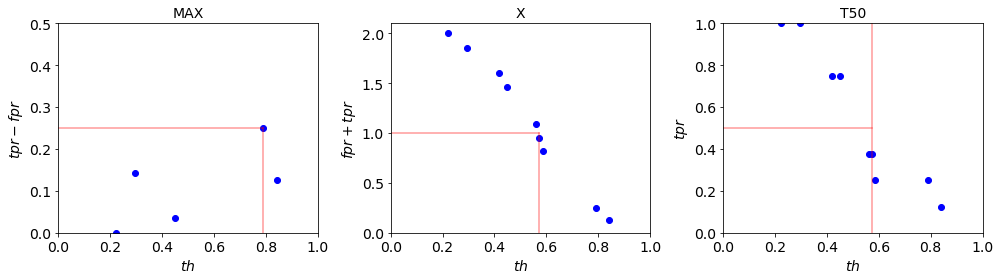
\includegraphics[width=\textwidth]{../plots_teoria/seleccion_umbrales_max_x_t50.png}
    \caption{}\label{fig:seleccion_umbrales_max_x_t50}
\end{figure}
Para el criterio MS, en cambio, por cada umbral que cambie $fpr$ o $tpr$ se
calcula una prevalencia (se descartan los casos indeterminados
por~\ref{ecuacion:acc_binaria}), y luego la mediana de todas ellas será la
prediccón final del método.
\begin{figure}[H]
    \centerline{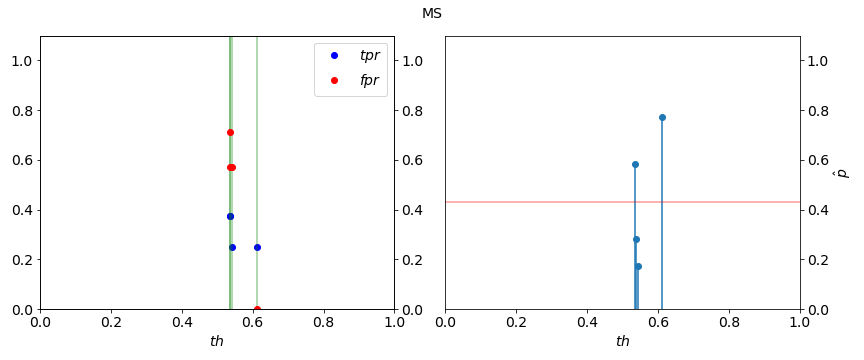
\includegraphics[width=0.75\textwidth]{../plots_teoria/seleccion_umbrales_ms.png}}
    \caption{}\label{fig:seleccion_umbrales_ms}
\end{figure}
Para los criterios MAX, X y T50, el resultado de~\ref{ecuacion:acc_binaria}
quedó negativo, por lo que las predicciones de las prevalencias de clases
incluyeron el truncamiento a 0, quedando $\hat p^{MAX}_{tst}(c=1)=\hat
p^{X}_{tst}(c=1)=p^{T50}_{tst}(c=1)=0$. Para el caso de $MS$, se obtuvo $\hat
p^{MS}_{tst}(c=1) \approx  0.46$.

\subsubsection{Esperanza-Maximización (EMQ)}\label{puntual:emq}

Aunque este método se propuso originalmente para mejorar las probabilidades {\it
a posteriori\/} de modelos de clasificación bajo {\it dataset shift\/}
(ver~\ref{problema:cambios}), el mismo también sirve para mejorar la estimación
de prevalencias. También conocido como {\it SLD\/} por las iniciales de sus
autores, este método fue propuesto por~\citet{saerens2002adjusting} y aplica el
agoritmo de Esperanza-Maximización (EM)~\cite{dempster1977maximum}, un conocido
algoritmo iterativo para encontrar estimaciones de máxima verosimilitud de
parámetros (los valores de prevalencia de clase) para modelos que dependen de
variables no observadas (las etiquetas de clase). Esencialmente, {\it EMQ\/}
actualiza incrementalmente las probabilidades {\it a posteriori\/} utilizando
los valores de prevalencia de clases calculados en el último paso de la
iteración, y actualiza los valores de prevalencia de clases utilizando las
probabilidades {\it a posteriori\/} calculadas en el último paso de la
iteración, de forma mutuamente recursiva, y tomando como punto de partida un
valor determinado para la prevalencia de clases (generalmente el valor
correspondiente a la muestra de entrenamiento o una estimación {\it a priori\/}
dada por algún conocimiento de la muestra de prueba, aunque puede ser cualquier
otro valor), y repitiendo las iteraciones hasta alcanzar la convergencia.

\citet[Apéndice, p.23 a p.25]{saerens2002adjusting} demuestra, mediante el
Teorema de Bayes y el Teorema de probabilidad total, que el algoritmo de EM
aplicado a este problema resulta en los siguientes pasos (el paso 0 se aplica
una sola vez, luego se iteran el E y M):

\begin{enumerate}[leftmargin=*, labelindent=16pt]

    \item[\bf{0 -}] Inicialización de $\hat p^{(0)}_{Y}(y=c_k)$, generalmente
    haciendo $\hat p^{(0)}_{Y}(y=c_k) = \hat p_{tr}(c=c_k)$

    \item[\bf{E -}] Esperanza: \hspace*{\fill}\makebox[4.5in][l]{$\hat
    p^{(s)}_{Y|\boldsymbol{X}=\boldsymbol{x}_i}(y=c_k) = \dfrac{\dfrac{\hat
    p^{(s)}_{Y}(y=c_k)}{\hat p_{tr}(c=c_k)}s(\boldsymbol{x}_i, y=c_k)}{\sum
    \limits_{j=1}^{\#C} \dfrac{\hat p^{(s)}_{Y}(y=c_j)}{\hat
    p_{tr}(c=c_j)}s(\boldsymbol{x}_i, y=c_k)}$}

    \item[\bf{M -}] Maximización: \hspace*{\fill}\makebox[4.5in][l]{$\hat
    p^{(s+1)}_{Y}(y=c_k)=\dfrac{1}{m}\sum \limits_{i=1}^{m}\hat
    p^{(s)}_{Y|\boldsymbol{X}=\boldsymbol{x}_i}(y=c_k)$}

\end{enumerate}

Finalmente, cuando se alcanza la convergencia, se obtiene: $\hat p^{\it EMQ
\/}_{tst}(c=c_k) = \hat p_{Y}(y=c_k)$.

Aunque ya mencionamos que el modelo supone que las probabilidades {\it a
posteriori\/} de modelos de clasificación ya están calibradas, se ha estudiado
también que el método {\it EMQ\/} mejora las predicciones de cuantificación si
el clasificador utilizado está calibrado~\cite{esuli2020critical,
alexandari2020maximum}.

\paragraph{\it Ejemplo:\/} Comenzamos con la inicialización, dando en nuestro
caso como resultado $\hat p^{(0)}_{Y}(y=1) = \hat p_{tr}(c=1) = 0.5$ y $\hat
p^{(0)}_{Y}(y=0) = \hat p_{tr}(c=0) = 0.5$. En la primera iteración, para el
paso E queda $\hat p^{(s=0)}_{Y|\boldsymbol{X}=\boldsymbol{x}_i}(y=c_k) =
s(\boldsymbol{x}_i, y=c_k)$ es decir, las mismas salidas del clasificador
calibrado. Luego, para el paso M, y al igual que en {\it PCC}, debemos promediar
cada salida individual del clasificador calibrado por cada una de las clases
existentes, quedando en nuestro caso $\hat p^{(s=1)}_{Y}(y=1) = p^{\it
PCC\/}_{tst}(c=1) \approx 0.45$. Ahora, en el paso E de la segunda iteración, se
usará este último valor junto con los valores de prevalencia de la muestra de
entrenamiento para ajustar las salidas del clasificador calibrado. Por ejemplo,
para ajustar la salida del primer invididuo correspondiente a la clase positiva,
sería: $\hat p^{(s=1)}_{Y|\boldsymbol{X}=\boldsymbol{x}_i}(y=1) \approx
\dfrac{\dfrac{0.45}{0.5}0.46}{\dfrac{0.45}{0.5}0.46+\dfrac{0.55}{0.5}0.54}$. Si
continuamos repitiendo los pasos E y M de forma sucesiva, y definiendo un
criterio de corte para la convergencia (ya sea por máxima cantidad de
iteraciones o por un umbral de diferencia entre $\hat p^{(s)}_{Y}(y=c_k)$ y
$\hat p^{(s+1)}_{Y}(y=c_k)$), se obtuvo $p^{\it EMQ \/}_{tst}(c=1) \approx 0$.

\subsubsection{Usando la distancia de Hellinger en $y$ (HDy)}\label{puntual:hdy}

\citet{gonzalez2013class} proponen dos métodos fundamentados en la comparación
de distribuciones. Aunque difieren en la manera de representar estas
distribuciones, ambos comparten un elemento esencial: emplean la distancia de
Hellinger como medida para cuantificar la disparidad entre ellas. El primer
método, conocido como {\it HDy}, es un método agregativo ya que emplea las
salidas del clasificador para describir las distribuciones tanto de la muestra
de entrenamiento como la de prueba. El método se basa en el cálculo de:
\begin{equation}\label{ecuacion:hdy}
    p^{\it HDy \/}_{tst}(c=1) = \argmin_{0 \leq \alpha \leq 1}{\text{HD}}(\alpha f_{tr}{(s(\boldsymbol{x},y=1|c=1))}+(1-\alpha) f_{tr}{(s(\boldsymbol{x},y=1|c=0))}, f_{tst}{(s(\boldsymbol{x},y=1))})
\end{equation}
donde:
\begin{equation}\label{ecuacion:hd}
    {\text{HD}}(P \parallel Q)= \frac{1}{\sqrt{2}}{\sqrt {\sum _{i=1}^{k}{({\sqrt {p_{i}}}-{\sqrt {q_{i}}})}^{2}}} \text{ con } P=(p_1,\dots,p_k), Q=(q_1,\dots,q_k)
\end{equation}
y $f_{tr}(s)$ y $f_{tst}(s)$ son las funciones de densidad de probabilidad de
las salidas del clasificador para la muestra de entrenamiento y de evaluación,
respectivamente. Estas densidades son aproximadas empíricamente mediante
histogramas, siendo $k$ el número de bins utilizados. Dado que el número de bins
$k$ podría tener un impacto significativo en la estimación, normalmente se
utiliza como estimador la mediana de la distribución de los $\alpha$ encontrados
para un rango de $k$.

El segundo método propuesto por~\citet{gonzalez2013class} pertenece a los
métodos no agregativos y será desarrollado en la correspondiente
sección~\ref{puntual:no_agregativos}.

\paragraph{\it Ejemplo:\/} En las siguientes gráficas vemos cómo son las
estimaciones de tres distribuciones estimadas para el ejemplo, la gráfica de la
función de costo usada, y cómo el mínimo encontrado se usa para combinar las
distribuciones de entrenamiento y compararlas con la de prueba. En este caso, se
utilizó sólo $k=100$.

\begin{figure}[h]
    \centering
    \begin{subfigure}[b]{\textwidth}
        \centering
        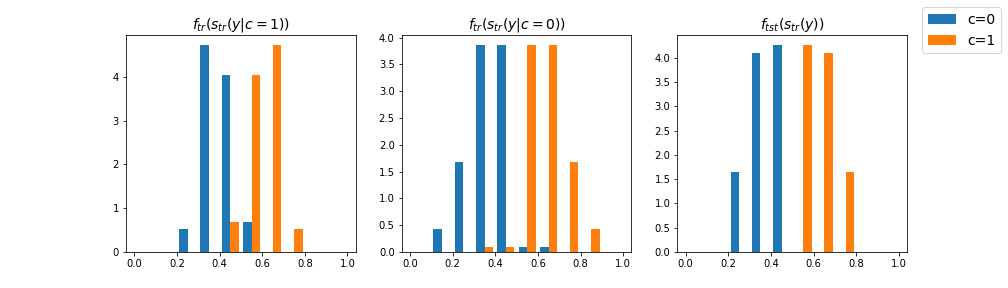
\includegraphics[width=\linewidth]{../plots_teoria/hdy_1.png}
    \end{subfigure}
    \begin{subfigure}[b]{0.4\textwidth}
        \centering
        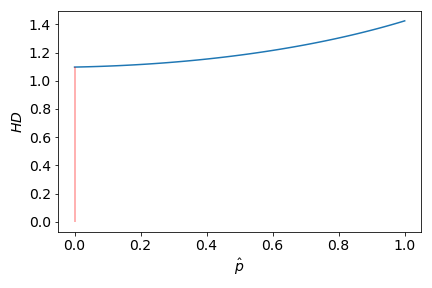
\includegraphics[width=\linewidth]{../plots_teoria/hdy_2.png}
    \end{subfigure}
    \begin{subfigure}[b]{\textwidth}
        \centering
        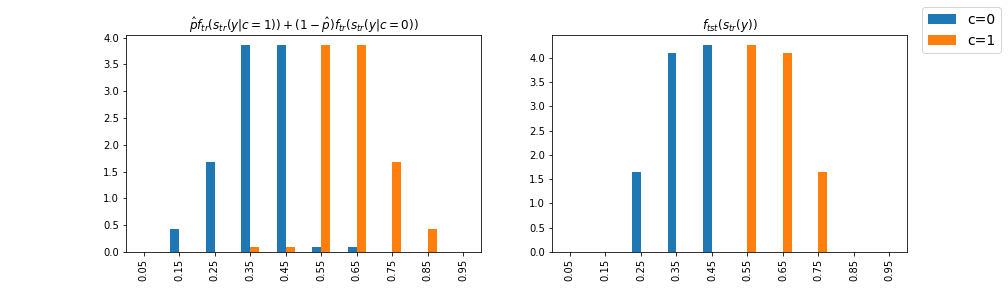
\includegraphics[width=\linewidth]{../plots_teoria/hdy_3.png}
    \end{subfigure}
    \hfill
\end{figure}

Se observa que el valor mínimo de HDy se da en $p^{\it HDy \/}_{tst}(c=1) =
0.34$.

\subsection{Con clasificadores específicos}\label{puntual:especificos}

Los métodos presentados anteriormente implican el uso de un clasificador, a
menudo seguido por una fase de ajuste para contrarrestar cualquier tendencia del
clasificador a subestimar o sobreestimar las proporciones de clases. Los
algoritmos discutidos en esta sección están específicamente diseñados con este
propósito en mente: durante el entrenamiento, tienen en cuenta que el modelo
será utilizado para cuantificar.

\subsubsection{Minimización de pérdida explícita (ELM)}\label{puntual:elm}

Esta familia de métodos se aplican en principio a la cuantificación binaria,
pero son fácilmente extensibles a la cuantificación multiclase. La idea
propuesta por Esuli y Sebastiani~\cite{esuli2010sentiment} es seleccionar una
medida de rendimiento de cuantificación y entrenar un algoritmo de optimización
para construir el modelo óptimo según esa medida. Las diferencias entre ellos se
deben a la medida de rendimiento seleccionada y al algoritmo de optimización
utilizado.

Esuli y Sebastiani~\cite{esuli2010sentiment, esuli2014explicit,
esuli2015optimizing} proponen utilizar ${\it SVM
\/}_{perf}$~\cite{joachims2005support} para optimizar la divergencia KL
-ver~\ref{evaluacion:dkl}-, mientras que~\citet{barranquero2015quantification}
también emplean ${\it SVM \/}_{perf}$ pero con una pérdida diferente,
argumentando que la cuantificación pura no considera la precisión del
clasificador subyacente (pudiendo generar un modelo que, aunque cuantifique
bien, clasifique mal). Para abordar esto, introducen la medida $Q$, que combina
una métrica de cuantificación con una métrica de clasificación, permitiendo un
equilibrio entre ellas.

Existen dos inconvenientes asociados con ${\it SVM \/}_{perf}$: podría resultar
en un modelo menos óptimo y no escala para grandes cantidades de datos de
entrenamiento. Para abordar estas limitaciones,~\citet{kar2016online} proponen
algoritmos de optimización estocástica. Además, plantean distintas métricas
multivariadas para evaluar el rendimiento de cuantificación. Siguiendo esta
línea,~\citet{sanyal2018optimizing} introducen una serie de algoritmos que
permiten el entrenamiento directo de redes neuronales profundas y la generación
de clasificadores no lineales. Estos métodos están diseñados para optimizar
funciones de pérdida de cuantificación como la divergencia KL.\@

\paragraph{\it Ejemplo:\/} A diferencia de los casos anteriores, aquí no usamos
el mismo clasificador con el que veníamos trabajando. En cambio, se ajusta un
nuevo clasificador pero con una función de pérdida más acorde al problema de
cuantificación. A modo de ejemplo, usaremos el método propuesto
por~\citet{esuli2010sentiment}, es decir, usando la divergencia KL como pérdida
y ${\it SVM \/}_{perf}$ como algoritmo de optimización. De esta forma, obtuvimos
un $p^{{\it SVM \/}_{perf}, {\it KLD \/}}_{tst}(c=1) \approx 0.44$, lo cual
efectivamente implica una mejora del KLD con respecto a usar el clasificador
anterior con {\it CC}, ya que ${\it KLD \/}^{\it CC\/}_{tst} \approx 0.55$ y
${\it KLD \/}^{{\it SVM \/}_{perf}, {\it KLD \/}}_{tst} \approx 0.28$.

\section{Métodos No Agregativos}\label{puntual:no_agregativos}

Hasta ahora, hemos utilizado métodos que agregan predicciones individuales de un
clasificador para poder cuantificar. Sin embargo, también es posible estimar
valores de prevalencia de clase sin generar decisiones binarias o probabilidades
{\it a posteriori\/} para cada ítem. Esta alternativa se fundamenta en el
principio de Vapnik, que sugiere resolver problemas directamente con la
información disponible en lugar de abordar un problema más general. En
cuantificación, esto significa que podemos estimar prevalencias de clase
directamente sin clasificar cada individuo.

\subsubsection{Usando la distancia de Hellinger en $\boldsymbol{x}$
(HDx)}\label{puntual:hdx}

Este método está obviamente relacionado con {\it HDy\/} (\ref{puntual:hdy}), con
la diferencia de considerar distribuciones de probabilidad multidimensionales
$f(\boldsymbol{x})$ en lugar de distribuciones unidimensionales $f(s(x))$.
Debido a la multidimensionalidad de $\boldsymbol{x} \in
\mathbb{R}^d$,~\citet{gonzalez2013class} proponen minimizar el promedio de las
divergencias de Hellinger por cada $\boldsymbol{x}^j$:

\begin{equation}\label{ecuacion:hdx}
    p^{\it HDx \/}_{tst}(c=1) = \argmin_{0 \leq \alpha \leq 1}{\frac{1}{d}\sum \limits_{j=1}^{d} \text{HD}}(\alpha f_{tr}({\boldsymbol{x^j}|c=1})+(1-\alpha) f_{tr}({\boldsymbol{x^j}|c=0}), f_{tst}({\boldsymbol{x^j}}))
\end{equation}

\paragraph{\it Ejemplo:\/} Repetimos el tipo de gráficos mostrados para  caso de
{\it HDy\/}, siendo en este caso $k=20$.

\begin{figure}[h]
    \centering
    \begin{subfigure}[b]{\textwidth}
        \centering
        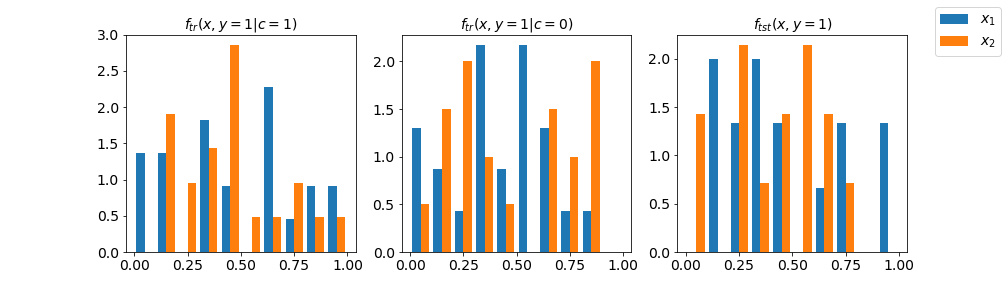
\includegraphics[width=\linewidth]{../plots_teoria/hdx_1.png}
    \end{subfigure}
    \begin{subfigure}[b]{0.4\textwidth}
        \centering
        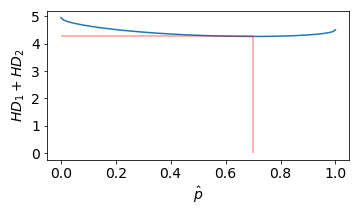
\includegraphics[width=\linewidth]{../plots_teoria/hdx_2.png}
    \end{subfigure}
    \begin{subfigure}[b]{\textwidth}
        \centering
        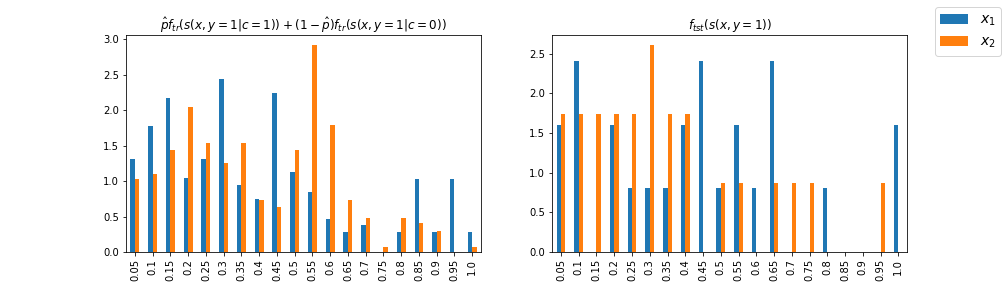
\includegraphics[width=\linewidth]{../plots_teoria/hdx_3.png}
    \end{subfigure}
    \hfill
\end{figure}

Se observa que el valor mínimo de HDx se da en $p^{\it HDx \/}_{tst}(c=1) =
0.23$.
